\section{Light rays deviation}

\begin{figure}[H]
    \centering
    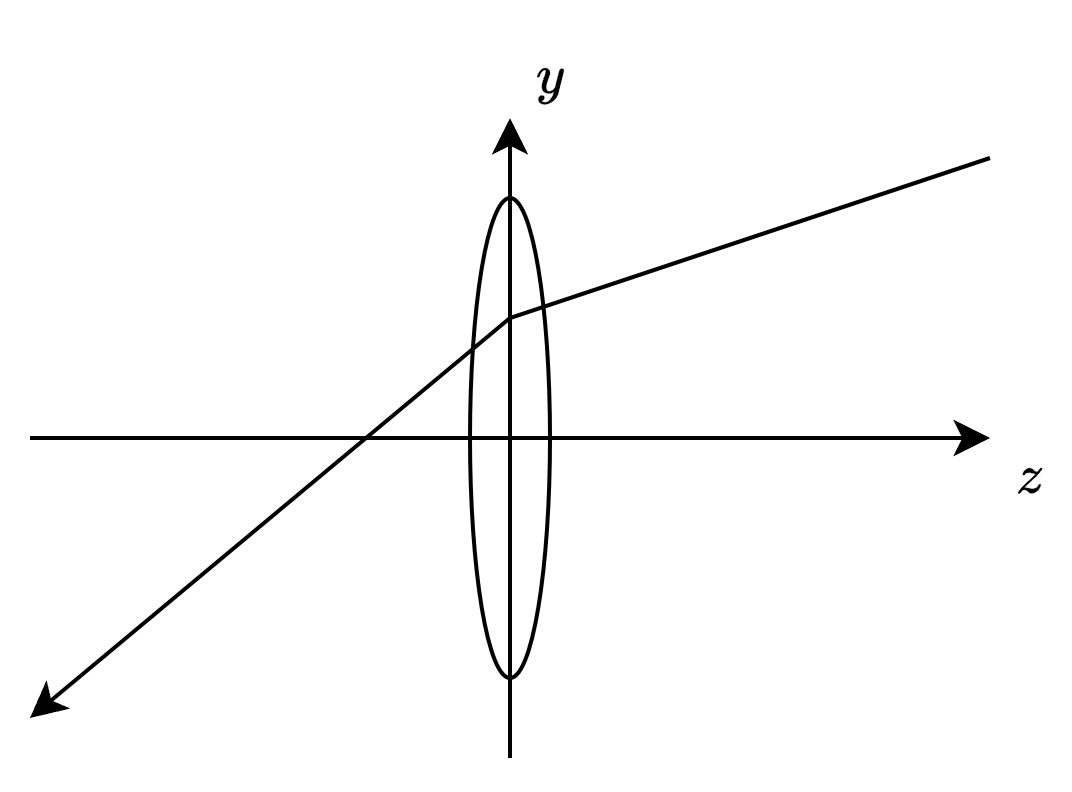
\includegraphics[width=0.4\linewidth]{images/ray.png}
\end{figure}
For a lens with a refractive index $n$, the following equations apply:
\[\dfrac{\theta-\alpha_1}{\theta^\prime-\alpha_1} \Rightarrow \dfrac{\sin{(\theta-\alpha_1)}}{\sin{(\theta^\prime-\alpha_1)}}=n\]
\[\dfrac{\theta^{\prime\prime}-\alpha_2}{\theta^\prime-\alpha_2} \Rightarrow \dfrac{\sin{(\theta^{\prime\prime}-\alpha_2)}}{\sin{(\theta^\prime-\alpha_2)}}=n\]
Here:
\begin{itemize}
    \item $\theta$ is the angle of the incoming ray before entering the lens.
    \item $\theta^\prime$ is the angle of the ray within the lens (not visible in the image).
    \item $\theta^{\prime\prime}$ is the angle of the ray after exiting the lens.
\end{itemize}
By comparing these two equations, we can express the difference between the input angle $\theta$ and the output angle $\theta^{\prime\prime}$ as:
\[\delta \theta=y(n-1)\left( \dfrac{1}{\rho_1} + \dfrac{1}{\rho_2}\right)\]
Here, the term $n-1$ reflects the influence of the lens material, while the term $\frac{1}{\rho_1} + \frac{1}{\rho_2}$ is determined by the curvature of the lens surfaces.